\section{Model process}
\label{sec:model_process}
This work deals with modeling of an open die forging process with multiple passes. The material used is a common stainless steel. The process parameters are orientated on a plan for forging a block with four passes given by the forging simulation software ForgeBase. Important process parameters, besides the flow curves, are for example the material data, the height reduction during every pass, the movement of the die, meaning the kinematics, the process temperature, etc. The detailed process conditions are discussed in the following chapters.\par

\subsection{Material data}
The material used is a 1.4301 (X5CrNiMo18-10) stainless steel. It is an austenitic steel which contains high quantities of the alloying elements chrome and nickel \ref{table:chemicalcomposition}. Therefore it is non-corrosive, acid- and heat-resistant. The field of application is widely spread and reaches from the automotive industry up to the chemical industry \cite{1.4301}.\par

The chemical composition (in weight-\%) of the material is as follows \cite{metallograf.de}:
\begin{table}[htbp]%[width=1.0\textwidth]
 \footnotesize
 \centering
 \caption{Chemical composition of 1.4301}
 \begin{tabular}{|c|c|c|c|c|c|c|c|}
 \hline
 C[\%]&Cr[\%]&Ni[\%]&Si[\%]&Mn[\%]&P[\%]&S[\%]&N[\%]\\\hline
 max 0,07&17,00-19,50&8,00-10,50&max 1,00&max. 2,00&max 0,045&max 0,03&max 0,11\\\hline
 \end{tabular}
 \label{table:chemicalcomposition}
\end{table}\par

For the input in a simulation model the thermal material data is crucial, containing are the temperature depending thermal conductivity, the spec. heat capacity and the Young´s modul, see figure \ref{img:thermalconductivity}, \ref{img:heatcapacity}, \ref{img:youngsmodul}. 

\begin{figure}[htbp]
 \centering
 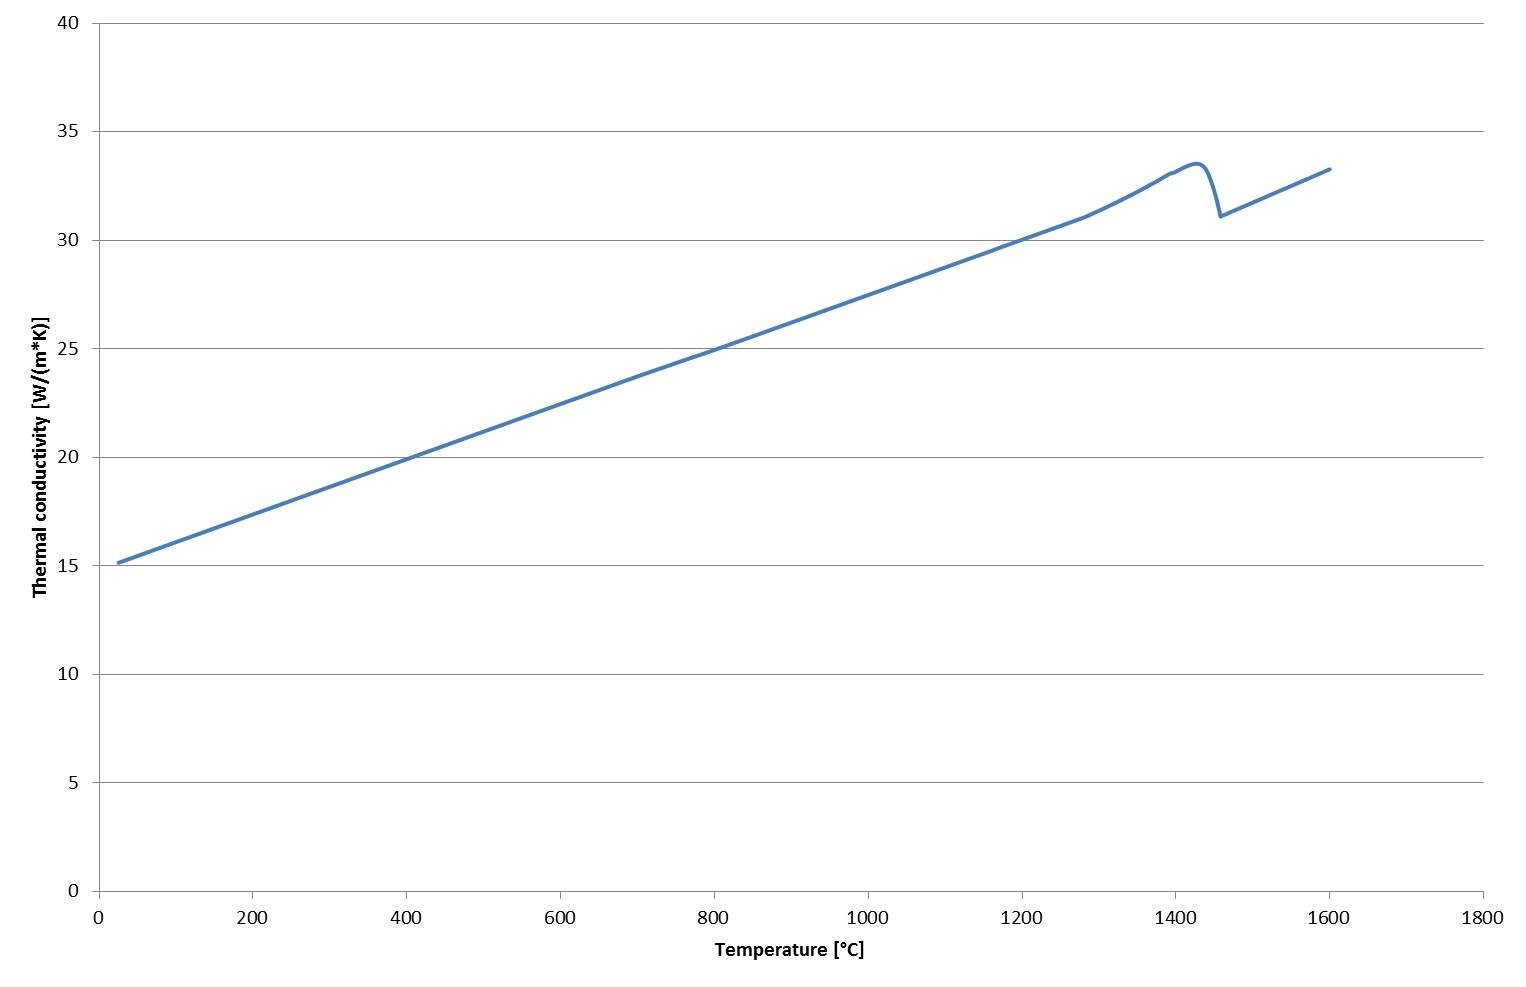
\includegraphics[width=0.8\textwidth]{images/thermalconductivity}
 \caption{Thermal conductivity of 1.4301}
 \label{img:thermalconductivity}
\end{figure}

\begin{figure}[htbp]
 \centering
 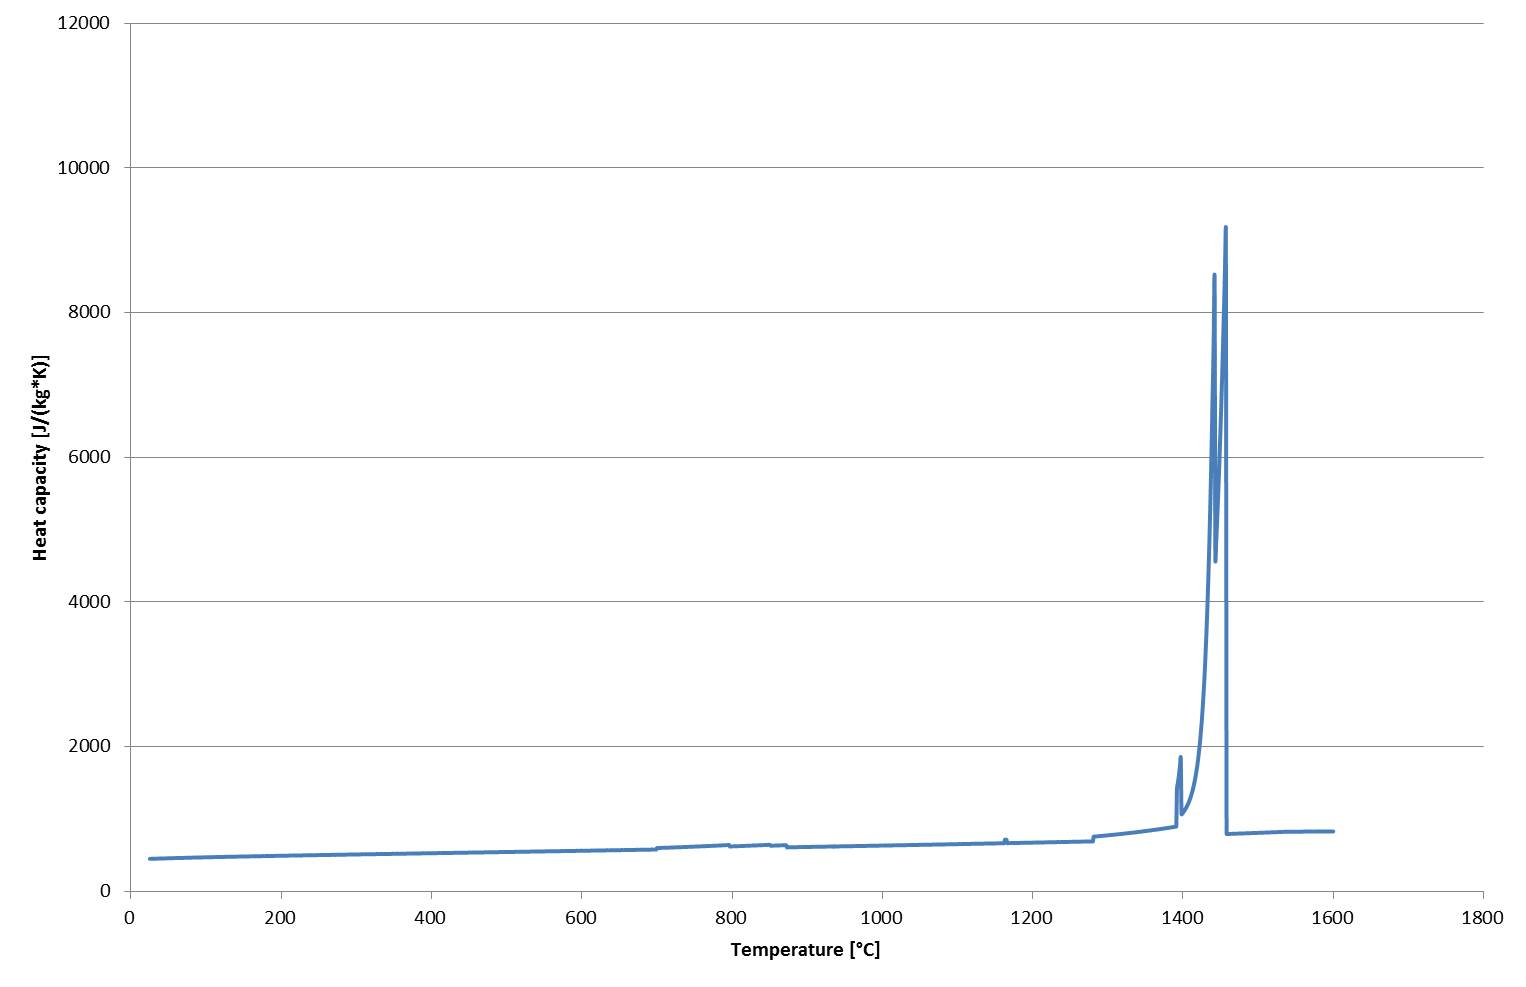
\includegraphics[width=0.8\textwidth]{images/heatcapacity}
 \caption{Heat capacity of 1.4301}
 \label{img:heatcapacity}
\end{figure}

\begin{figure}[htbp]
 \centering
 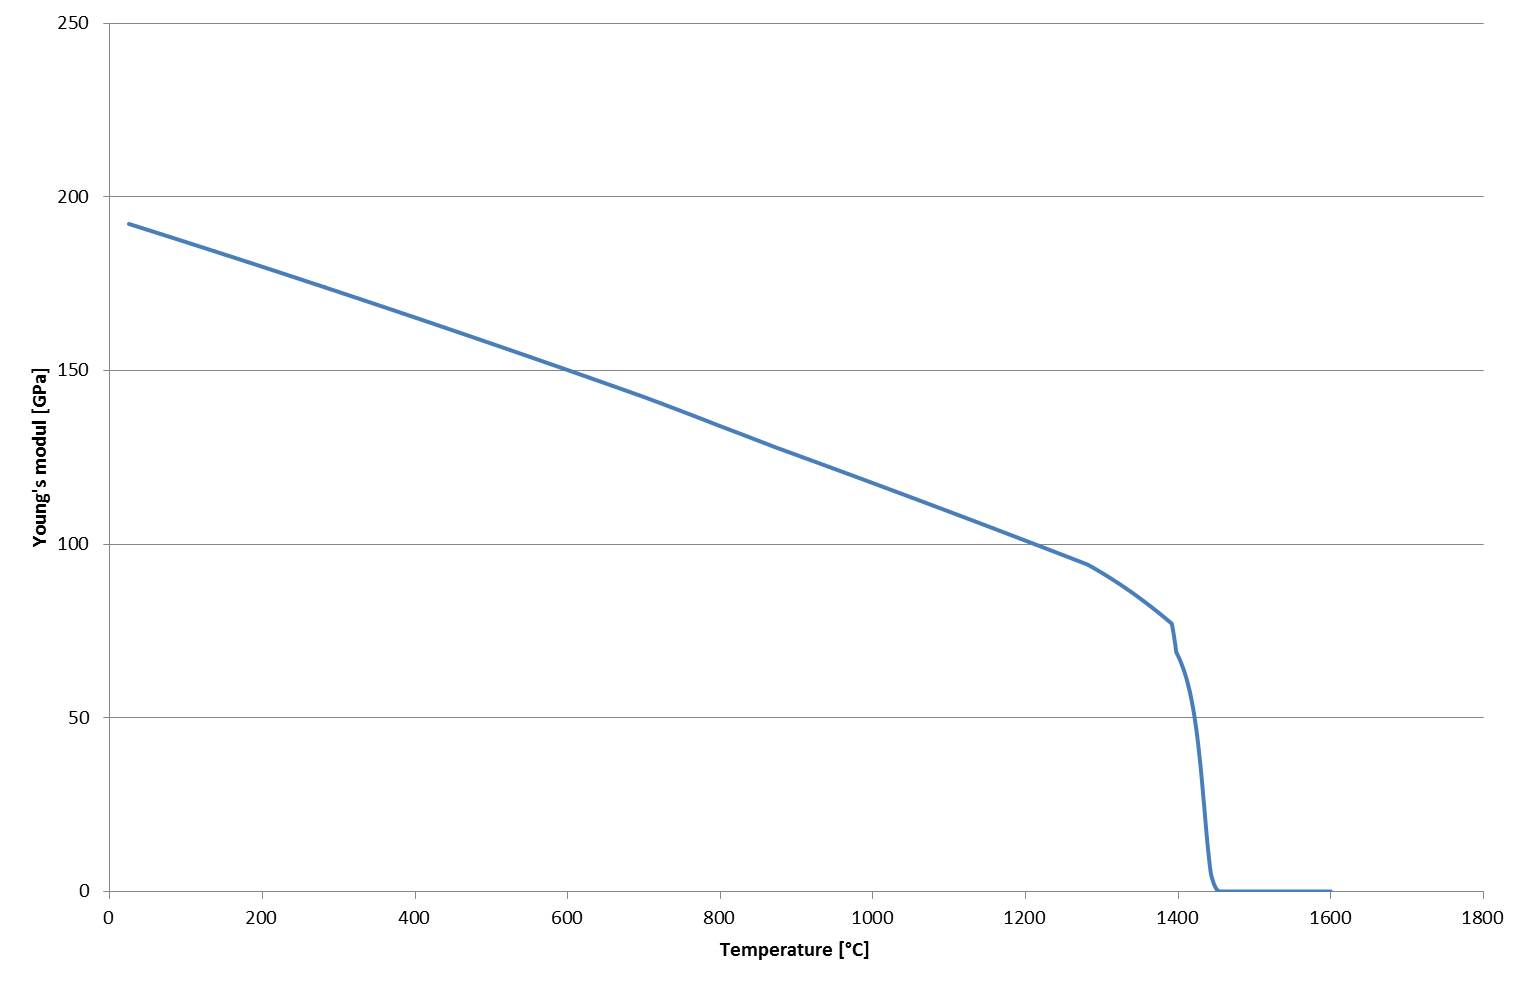
\includegraphics[width=0.8\textwidth]{images/youngsmodul}
 \caption{Young's modul of 1.4301}
 \label{img:youngsmodul}
\end{figure}

It is necessary that the data describes the whole temperature range of the process. Further parameters are set constant and are pictured in \ref{table:processparameter}. 

\begin{table}[htbp]%[width=0.8\textwidth]
 \centering
 \caption{Constant process parameters (reference temperature 20°C)}
 \begin{tabular}{|c|c|c|}
 \hline
 Poison&0,3&-\\
 \hline
 Thermal expansion&0,000012&[1/K]\\
 \hline
 Emissivity&0,7&-\\
 \hline
 Heat transfer coeff.&4,5&[W/(m²K)]\\
 \hline
 Friction coeff.&0,4&-\\
 \hline
 Dissipation&0,9&\%\\
 \hline
 \end{tabular}
 \label{table:processparameter}
\end{table}

\subsection{Forging plan (ForgeBase)}
The settings of the forging simulation are based on the calculation of the forging software ForgeBase \ref{table:forgingplan}. The simulations are done for a four passes process on a block (workpiece - WP) with the dimensions of 150mm in height as well as in width and 600mm in length. However, only 400mm of the length are forged. The rest is provided for the manipulator to hold and move the WP. The WP is set as a plastic solid and is meshed with a brick mesh with 12544 elements. The upper and lower dies are set as rigid object. The manipulator is set up as a spring with a stiffness of 175 N/mm and the maximum clamping force of 222,4 kN.\par 

The passes in the simulation vary in height reduction and bite ratio. Between the passes the WP is rotated in positive and negative direction with 90° rotation angle. There are two models of movement. On the one hand the bottom die is fixed, though the top die moves with a speed of 80mm/s (Simufact). On the other hand the top and the bottom die move with a speed of 40mm/s (DEFORM; PEP/LARSTRAN).

\begin{figure}[htbp]
 \centering
 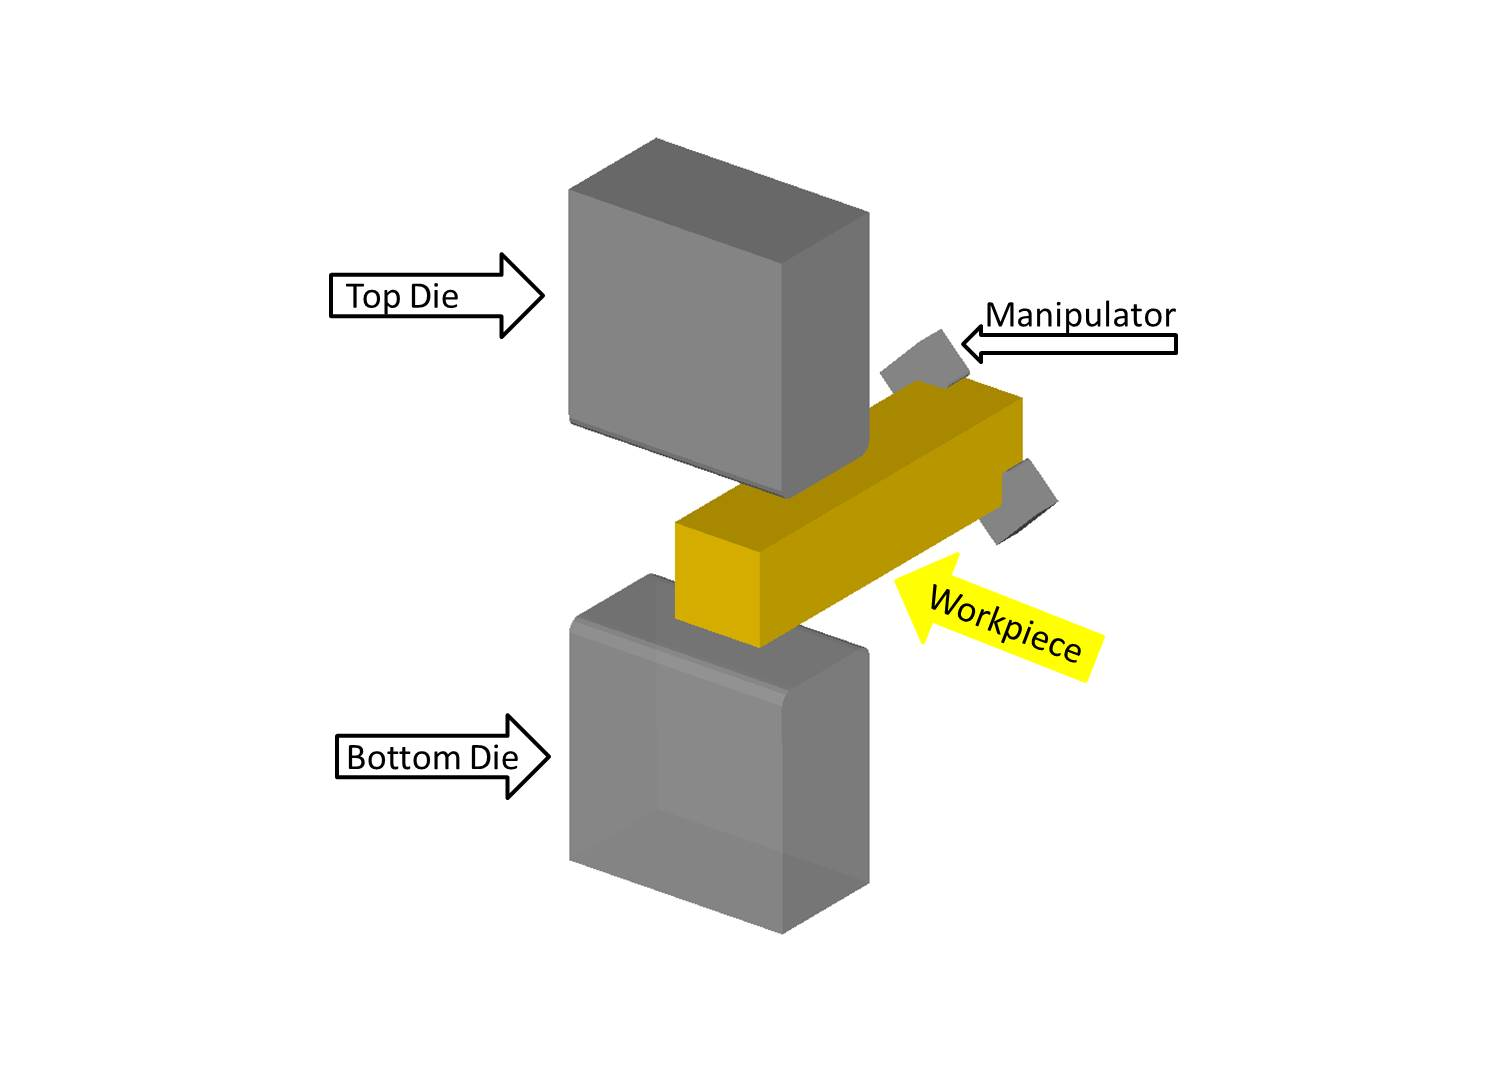
\includegraphics[width=0.8\textwidth]{images/processsetup}
 \caption{Illustration of the process setup from DEFORM}
 \label{img:processsetup}
\end{figure}

\begin{table}[htbp]%[width=1\textwidth]
 \footnotesize
 \centering
 \caption{Forging plan from ForgeBase}
 \begin{tabular}{|c|c|c|c|c|c|c|c|}
 \hline
 Pass Nr.&Reduction&Height 1&Width 1&Height 2&Width 2&Rotation&Bite width\\
 & [mm] & [mm] & [mm] & [mm] & [mm] & [$^{\circ}$] & [mm]\\
 \hline
 0&0&150&150&150&150&0&0\\
 \hline
 1&28&122&162&122&162&0&105\\
 \hline
 2&30&132&132&132&132&90&85\\
 \hline
 3&25&107&143&107&143&-90&92\\
 \hline
 4&27&116&116&116&116&90&75\\
 \hline
 \end{tabular}
 \label{table:forgingplan}
\end{table}

Moreover, the heat treatment before and during the process is of great importance. Before the first pass starts, the WP gets heated up to 1200°C for 2 hours. It is vital, that the WP does have a homogeneous distribution. During the forging passes, heat is getting lost by the effects of emission and the heat transfers to the dies. Because of that, a second heat is necessary between the second and the third pass. The WP is heated up again to 1200°C within 1 hour. After the last pass the WP cools down upon air to room temperature.
